\chapter{Modelos SARIMA}

\section{Identificaci�n del modelo}

Antes de realizar la proyecci�n de una serie de tiempo, es necesario identificar el modelo que explique adecuadamente su comportamiento. 

Aunque conocemos, por la estrucutura del proceso que genera los datos, que las series de tiempo de poblaci�n sindicada y condenada no son independientes, podemos simplificar la proyecci�n, trat�ndolas como independientes. En este caso, los modelos ARIMA y SARIMA resultan apropiados, pues permiten explicar separadamente cada observaci�n en funci�n del comportamiento hist�rico de la serie.

El cap�tulo anterior suger�a que la poblaci�n carcelaria, tanto sindicada como condenada, tiene una marcada tendencia al alza. En este caso una herramienta �til es graficar la variaci�n mes a mes de la poblaci�n. \ref{fig:variacion_intermensual}. Para tener una mejor estrucutura de an�lisis usamos la funci�n "decompose" de R base. 

La serie tiene un componente estacional marcado, con una reducci�n de la poblaci�n carcelaria en diciembre. La variabilidad del componente aleatorio es elevada. La tendencia parece tener cambios estructurales en algunos periodos, por ejemplo reducci�n de la poblaci�n carcelaria entre 2005-2007,  y 2012 - 2015, e incrementos de la poblaci�n de magnitud mayor al promedio entre 2008 y 2012.

La mayor parte de la variaci�n de la poblaci�n total, se puede asociar con variaciones en a poblaci�n sindicada \ref{fig:variacion_mensual_sindicados_desc}. La poblaci�n condenada tiene una tendencia con una tendencia m�s estable.  \ref{fig:variacion_mensual_condenados_desc}


\begin{figure}
	\centering
	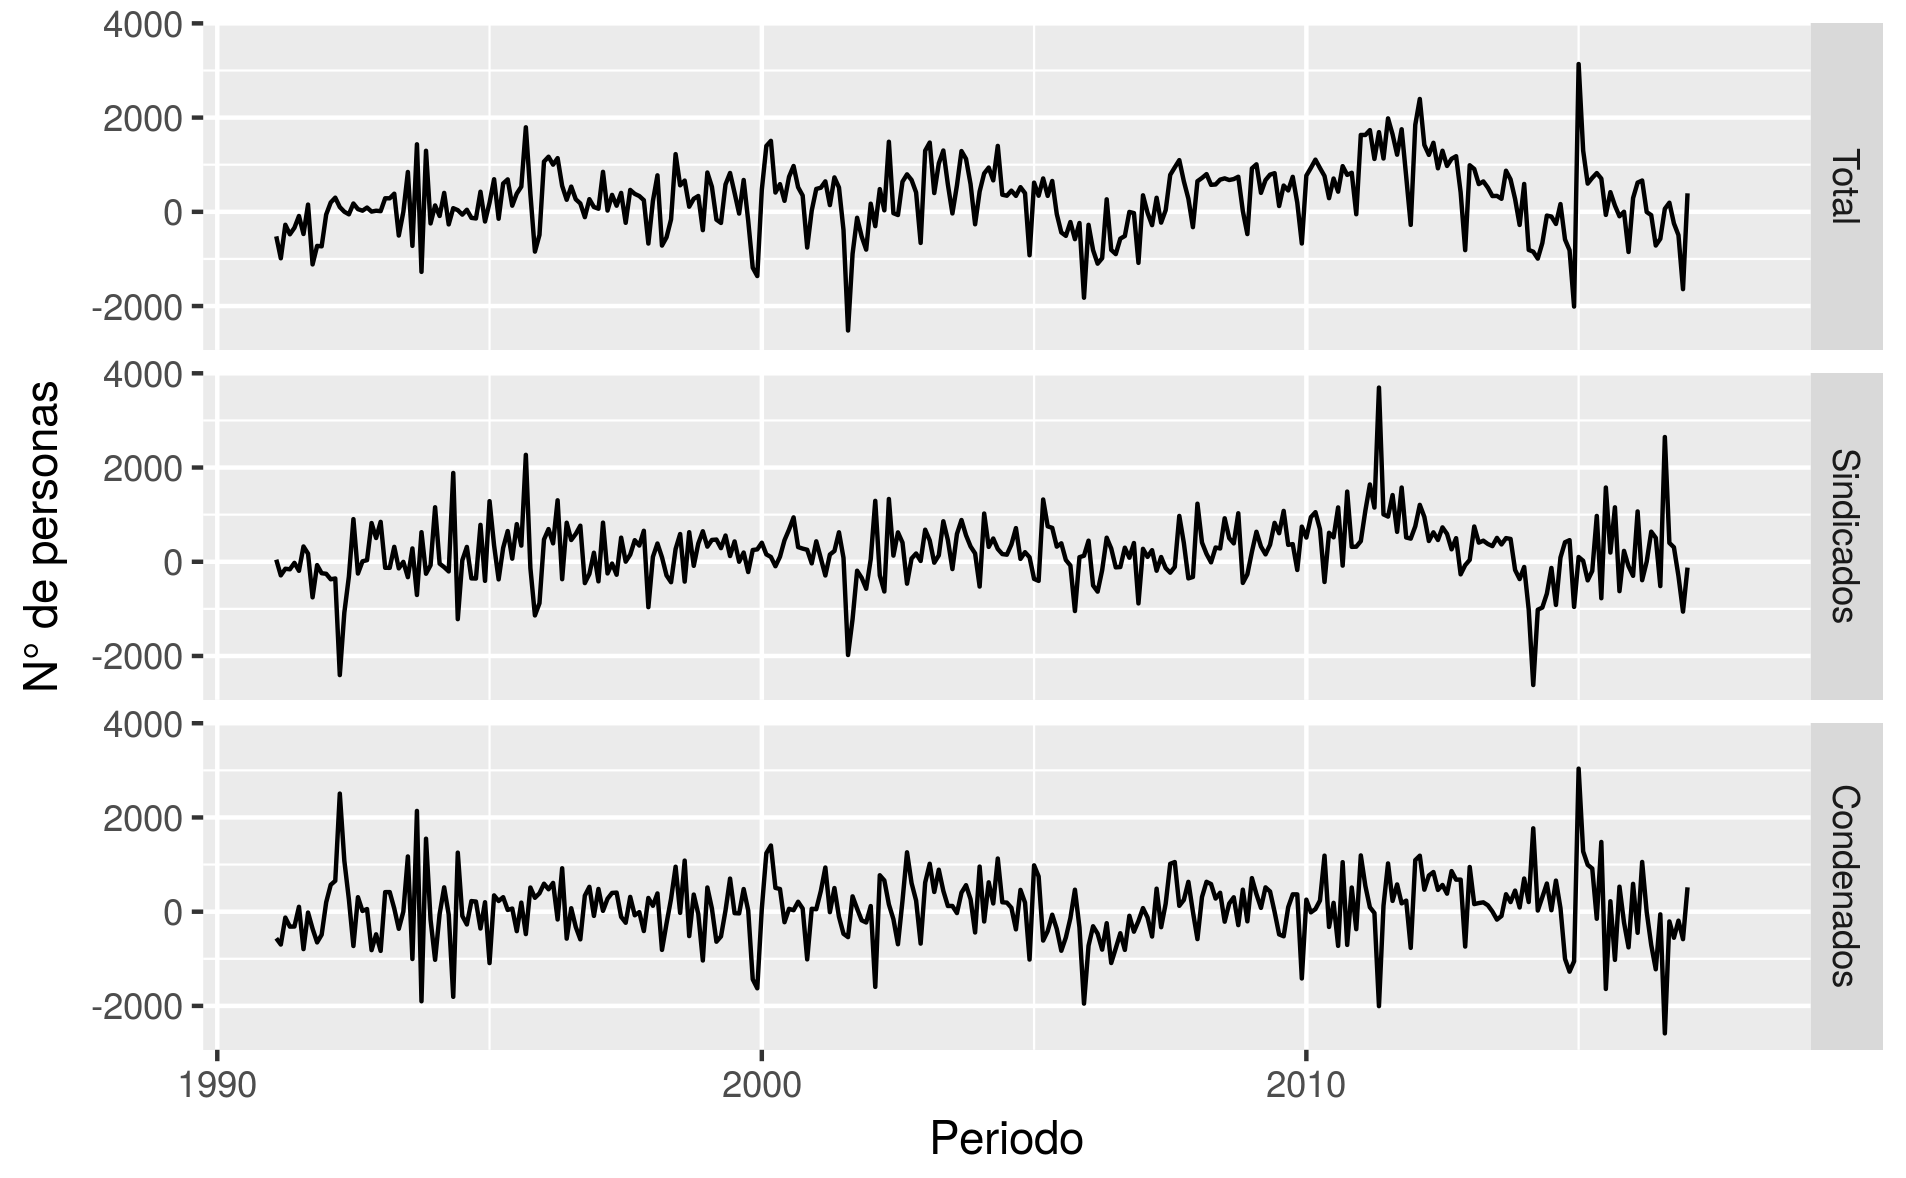
\includegraphics[width=0.7\linewidth]{variacion_intermensual}
	\caption[Variaci�n inter-mensual de poblaci�n carcelaria]{Variaci�n inter-mensual de poblaci�n carcelaria, sindicados y condenados}
	\label{fig:variacion_intermensual}
\end{figure}


\begin{figure}
\centering
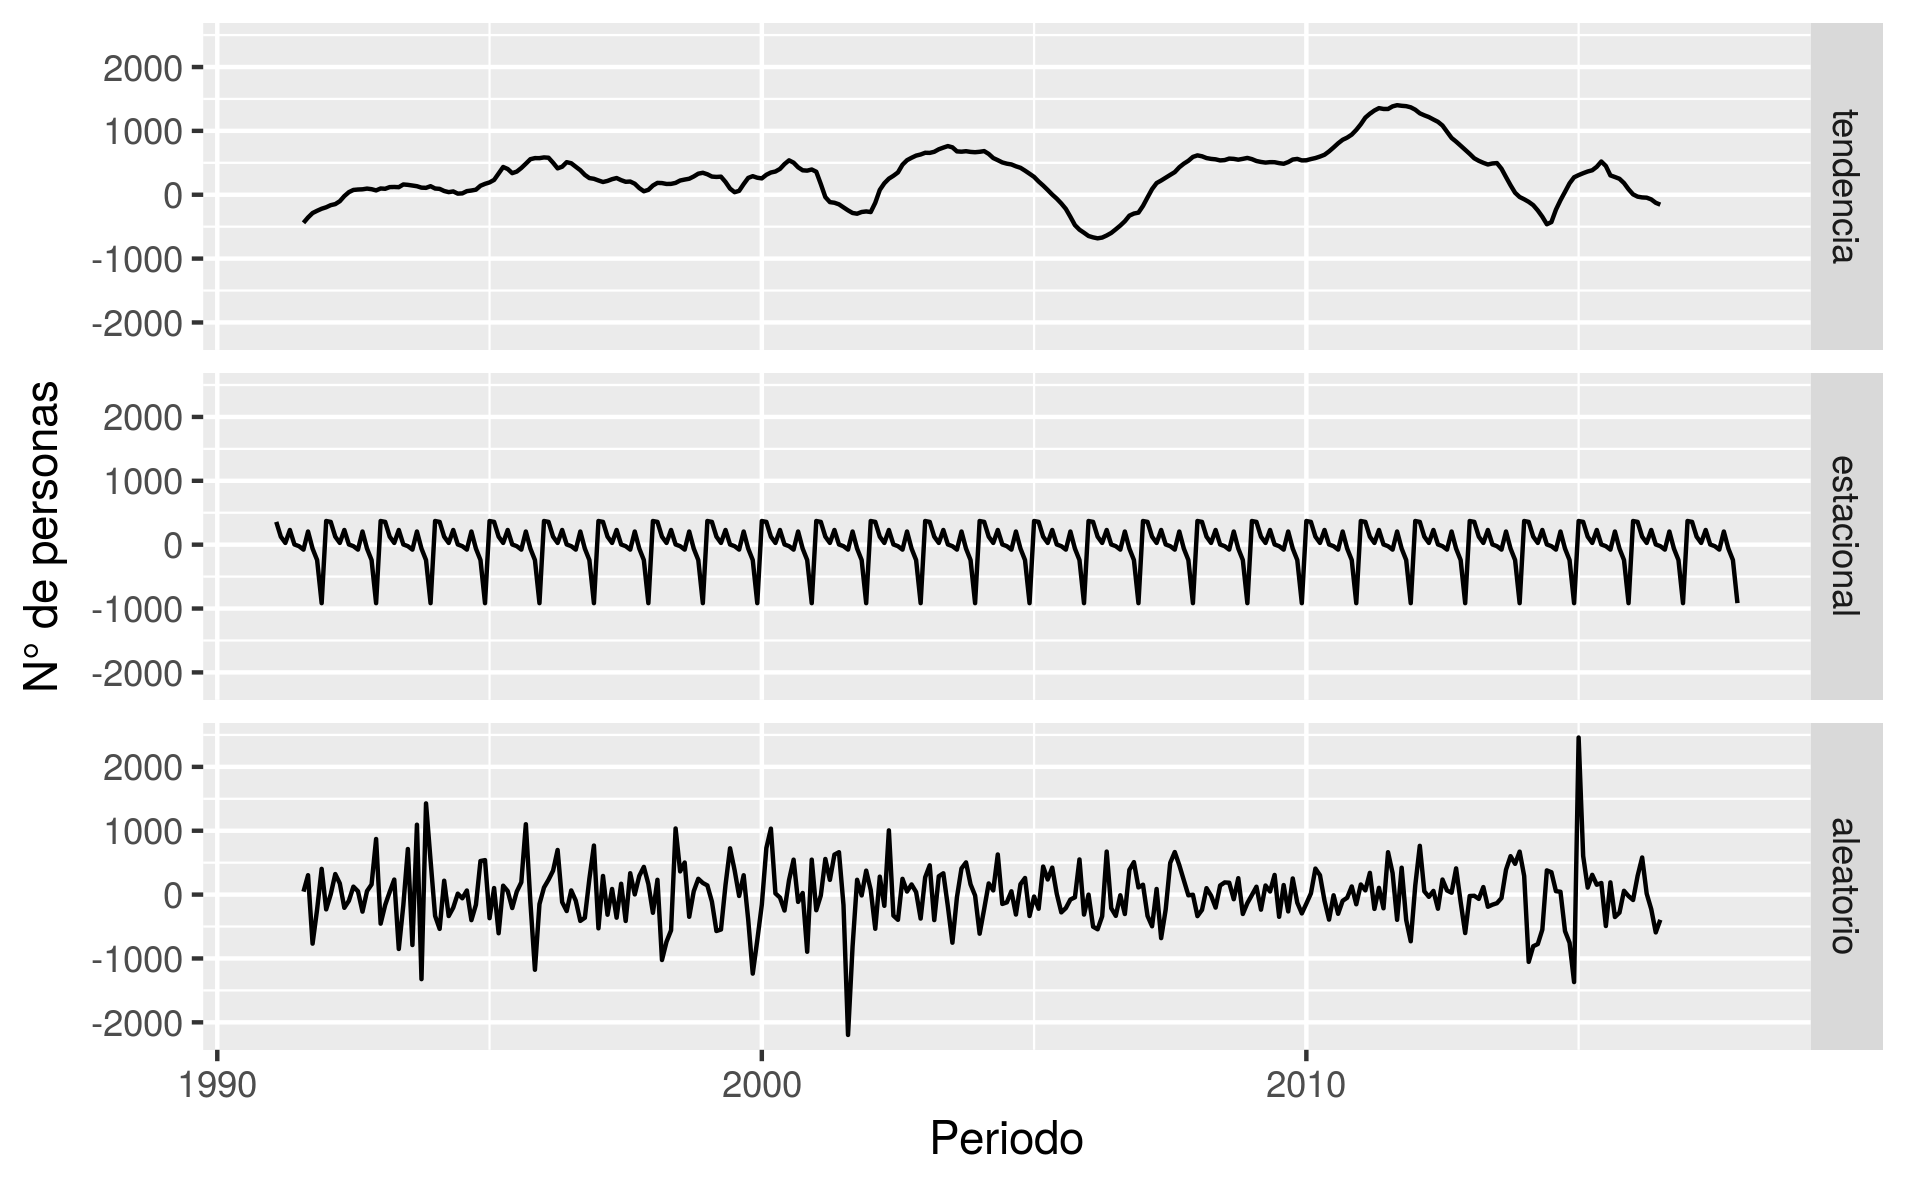
\includegraphics[width=0.7\linewidth]{variacion_mensual_total_desc}
\caption[Descomposici�n de la variaci�n inter-mensual de poblaci�n carcelaria total]{Variaci�n mensual de poblaci�n carcelaria descompuesta por tendencia, estacionalidad y componente aleatorio.}
\label{fig:variacion_mensual_total_desc}
\end{figure}

\begin{figure}
	\centering
	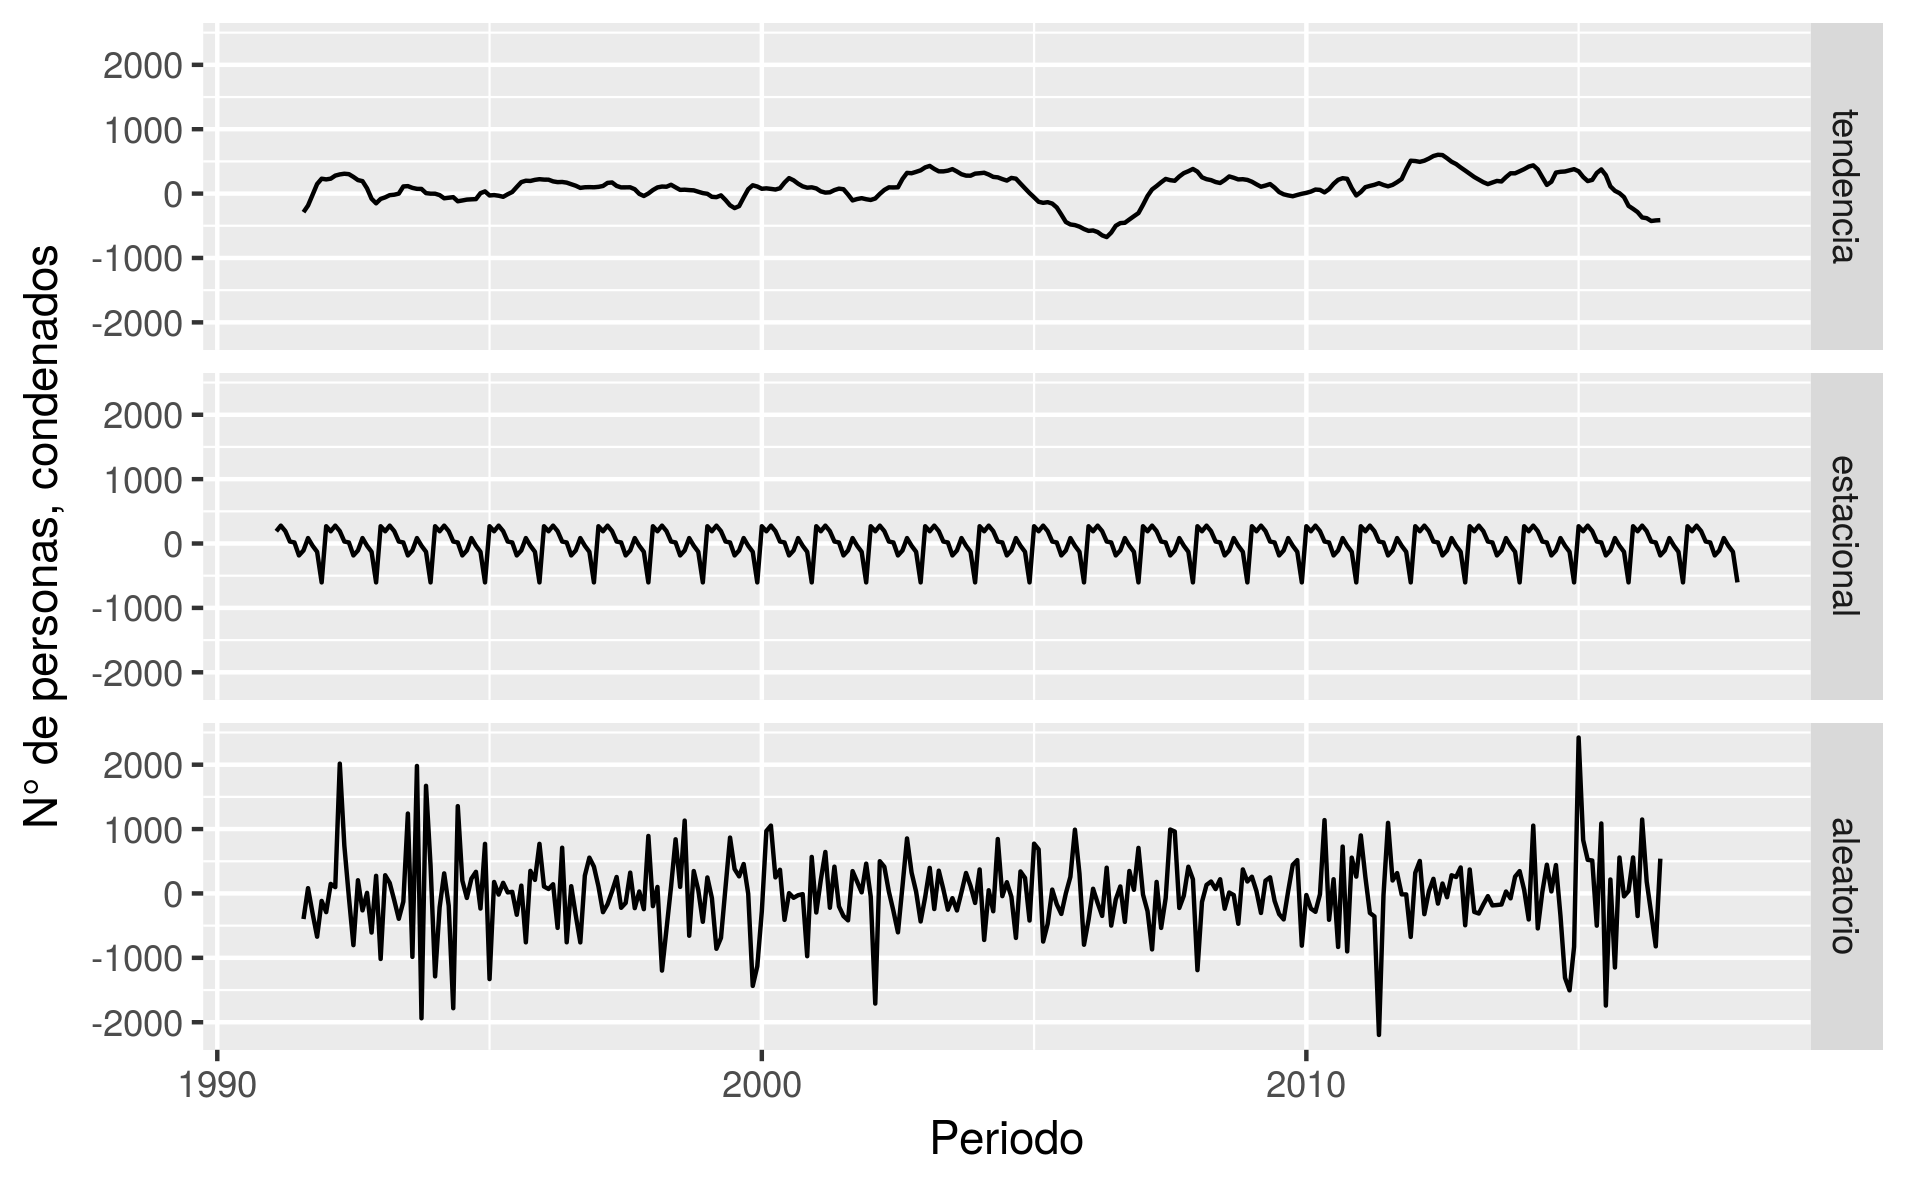
\includegraphics[width=0.7\linewidth]{variacion_mensual_condenados_desc}
	\caption[Descomposici�n de la variaci�n inter-mensual de poblaci�n carcelaria total]{Variaci�n mensual de poblaci�n carcelaria sindicada,  descompuesta por tendencia, estacionalidad y componente aleatorio.}
	\label{fig:variacion_mensual_condenados_desc}
\end{figure}

\begin{figure}
	\centering
	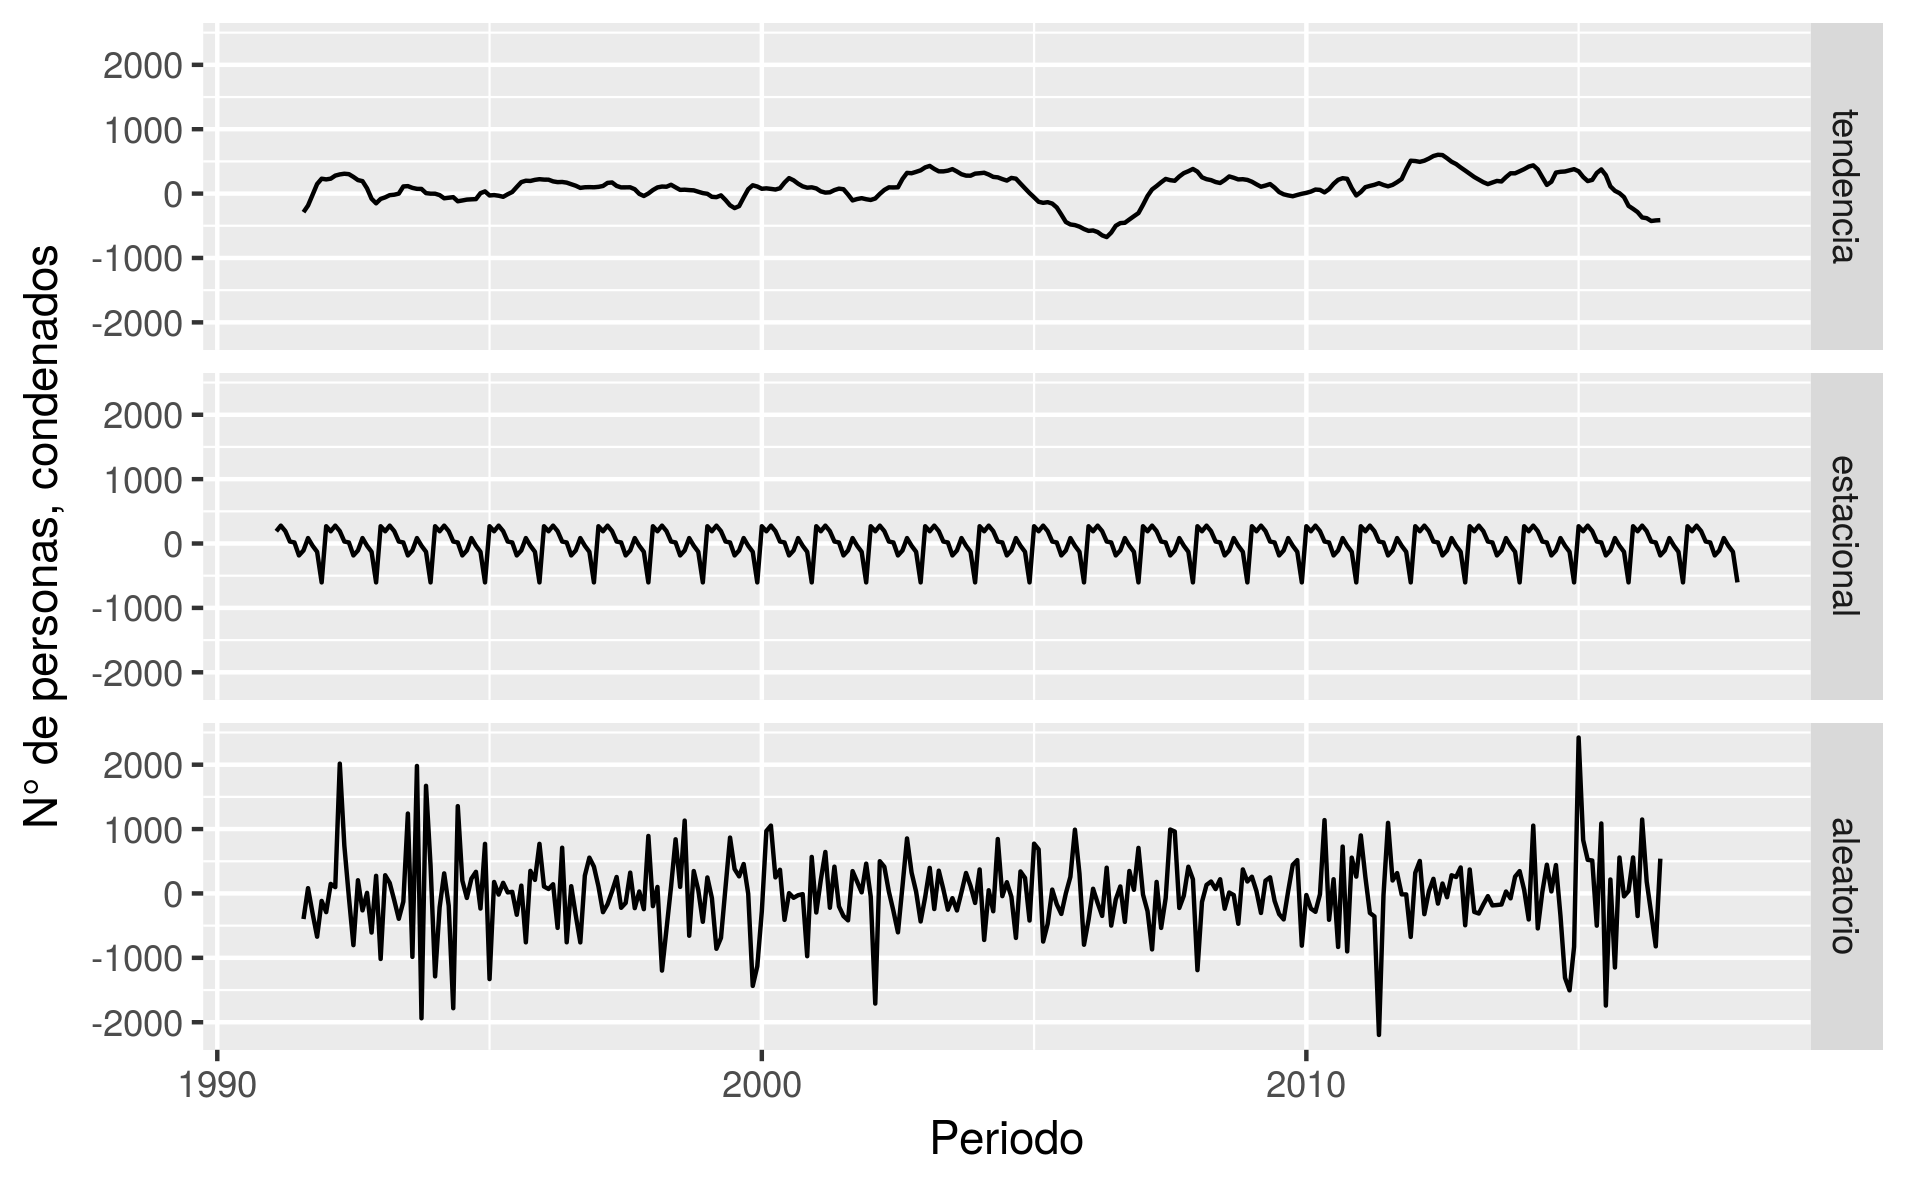
\includegraphics[width=0.7\linewidth]{variacion_mensual_condenados_desc}
	\caption[Descomposici�n de la variaci�n inter-mensual de poblaci�n carcelaria condenada]{Variaci�n mensual de poblaci�n carcelaria condenada,  descompuesta por tendencia, estacionalidad y componente aleatorio.}
	\label{fig:variacion_mensual_sindicados_desc}
\end{figure}



\section{Proyecciones 2017 - 2020}

\section{Conclusiones}